\documentclass[11pt]{article} 
\usepackage[margin=1in]{geometry} 
\usepackage{amsfonts,amsmath,amssymb,graphicx,color}
\usepackage{mathtools}
\usepackage{psfrag} 
\usepackage{pdflscape} 
\usepackage{soul} 
\usepackage{algorithm} 
\usepackage{algpseudocode} 
\usepackage{hyperref} 
\usepackage{multirow} 
\usepackage{caption} 
\usepackage{subcaption} 
\usepackage{showlabels}
\usepackage{appendix}
\usepackage[T1]{fontenc} 

\newtheorem{thm}{Theorem}

\newcommand{\defeq}{\stackrel{\rm def}{=}}
\newcommand{\defeqq}{\vcentcolon=}
\newcommand{\Var}{\mathrm{Var}}

\renewcommand{\theequation}{\thesection.\arabic{equation}}
\newcommand{\comment}[1]{}

\setcounter{section}{0}


\title{Memory Reduction Techinques for Aggregated Gradient Methods}

\begin{document}
\newpage

\section{Intro}

	Two popular aggregated gradient methods, SAG and SAGA, require storing $m$ past gradients in memory. When $m$ is large, this might be infeasible. In fact, consider a dense multi-class logistic regression problem with L2 regularization. For $m$ datapoints, $c$ classes, and $k$ features, the total data storage is $m k$, while storing all gradients requires $mck$ storage. We suggest and evaluate various memory reduction techniques for aggregated gradient methods.
	
\subsection{Chunking}

The chunking idea is to split up the data into $K$ chunks, and run the aggregated gradient methods as usual, but using the chunks as the new datapoints. Thus every iteration requires $\frac{m}{K}$ sample gradient evaluations instead of one evaluation in the original aggregated gradient methods, but requires storing $K$ sample gradient averages instead of $m$. The special cases are:
\begin{itemize}
	\item $K=m$ gives the original SAG/SAGA method
	\item $K=1$ gives the batch gradient descent method
	\item $1<K<m$ area of interest, chunking methods
\end{itemize}
\includegraphics{Figures/Chunking.pdf}
	
		Assume that $s_k$ is divisible by $C$ for every $k$. In this case, we can introduce the concept of chunking, or mini-batch replacement and storing. Instead of storing the values of each $ \nabla f_j(\phi_j^k)$, we store appropriate sample gradient averages $\frac{1}{m} \sum_{i=1}^m  \nabla f_i(x)$.

	\begin{algorithm}
		[H] 
		\caption{SAG - Chunking}
		\label{alg:sag-chunking}
		{\bf Input:} Initial iterate $\theta^0$, number of chunks $C$, $\{ \alpha_k \}$, number of datapoints $m$
		\begin{algorithmic}
			[1] 
			\State Initialize $g_i^{-1} = \frac{C}{m} \sum_{j \in \mbox{chunk } i }  \nabla f_{j}(\theta^0) $
			\Loop { $k= \{ 0,1,\ldots \}$}
			\State Sample $i$ from $\{ 1, \ldots, C \}$
			\State $ g_i^k = \frac{C}{m} \sum_{j \in \mbox{chunk } i }  \nabla f_{j}(\theta^k) $ 
			\State $ g_j^k = g_j^{k-1} $ for $j \neq i$ 
			\State $g^k = \frac{1}{C} \sum_{j=1}^C g_j^k$ 
			\State $\theta^{k+1} = \theta^k - \alpha_k g^k$ 
			\EndLoop 
		\end{algorithmic}
	\end{algorithm}


	\begin{algorithm}
		[H] 
		\caption{SAGA - Chunking}
		\label{alg:saga-chunking}
		{\bf Input:} Initial iterate $\theta^0$, number of chunks $C$, $\{ \alpha_k \}$, number of datapoints $m$
		\begin{algorithmic}
			[1] 
			\State Initialize $g_i^{-1} = \frac{C}{m} \sum_{j \in \mbox{chunk } i }  \nabla f_{j}(\theta^0) $
			\Loop { $k= \{ 0,1,\ldots \}$}
			\State Sample $j$ from $\{ 1, \ldots, C \}$
			\State $g_i^k = \frac{C}{m} \sum_{j\in \mbox{chunk } i }  \nabla f_{j}(\theta^k) $ 
			\State $ g_j^k = g_j^{k-1} $ for $j \neq i$ 
			\State $g^k =  g_i^{k} -  g_i^{k-1}  + \frac{1}{C} \sum_{j = 1}^{C}g_j^{k-1}$ 
			\State $\theta^{k+1} = \theta^k - \alpha_k g^k$ 
			\EndLoop 
		\end{algorithmic}
	\end{algorithm}
	
\subsection{Representative Storage}

The data must be split up into groups, preferably with samples in each group similar to each other. Sampling is still done on the whole dataset, but the replacement in memory is done by group, not by every datapoint. 

\includegraphics{Figures/Representative.pdf}

	
\subsection{Re-Evaluate Instead of Store}

If historical $\theta$ points are stored, then any sample gradients can be re-evaluated at that point. Thus a SAGA-SVRG continuum can be achieved.

\includegraphics{Figures/StoreTheta.pdf}

Instead of $\tilde{x}$, save a few $\tilde{\theta_{c(j)}}$. This reduces the storage of saga from $m$ vectors to however many chunks are chosen.
This method creates a continuum between SAGA and SVRG (these are limiting cases). 
\[ \nabla f_j(\theta^k) -  \nabla f_j(\tilde{\theta_{c(j)}}) + \frac{1}{m}\sum_{i=1}^{m}  \nabla f_i (\tilde{\theta_{c(j)}})\]
	
\subsection{Evolving Gradient Methods}




\section{Numerical Experiments}
\subsection{Chunking}
	The following experiments show the algorithm progress after 40 passes over the data. Only two types of chunking are tested: SAG and SAGA chunking. The labels are in the format \texttt{algorithm numChunks StepsizePower}. The stepsizes were tuned to give the best final function value. 
     
		 \newpage
	 
	\includegraphics[width= 5in]{Figures/agaricusBLtruefchunking.pdf}

	\includegraphics[width= 5in]{Figures/agaricusBLtruemccchunking.pdf}

	\includegraphics[width= 5in]{Figures/myrandBLtruefchunking.pdf}

	\includegraphics[width= 5in]{Figures/myrandBLtruemccchunking.pdf}

	\includegraphics[width= 5in]{Figures/MNISTBLtruefchunking.pdf}

	\includegraphics[width= 5in]{Figures/MNISTBLtruemccchunking.pdf}

	\includegraphics[width= 5in]{Figures/alphaGoodBLtruefchunking.pdf}

	\includegraphics[width= 5in]{Figures/alphaGoodBLtruemccchunking.pdf}


	\subsection{Representative}

	\includegraphics[width= 5in]{Figures/MNISTBLtruefCB.pdf}

	\includegraphics[width= 5in]{Figures/MNISTBLtruemccCB.pdf}

	\includegraphics[width= 5in]{Figures/myrandBLtruefCB.pdf}

	\includegraphics[width= 5in]{Figures/myrandBLtruemccCB.pdf}

	\includegraphics[width= 5in]{Figures/agaricusBLtruefCB.pdf}

	\includegraphics[width= 5in]{Figures/agaricusBLtruemccCB.pdf}

	\includegraphics[width= 5in]{Figures/alphaGoodBLtruefCB.pdf}

	\includegraphics[width= 5in]{Figures/alphaGoodBLtruemccCB.pdf}
	
	\subsection{Store Theta}
	
	
	\subsection{Evolving Gradient}

	\includegraphics[width= 5in]{Figures/agaricusBLtruefInitialHeuristics.pdf}

	\includegraphics[width= 5in]{Figures/agaricusBLtruemccInitialHeuristics.pdf}

	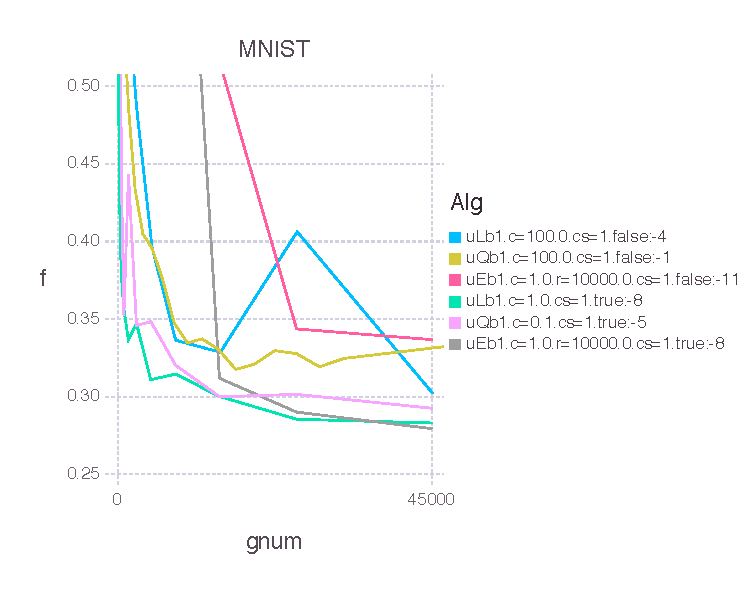
\includegraphics[width= 5in]{Figures/MNISTBLtruefInitialHeuristics.pdf}

	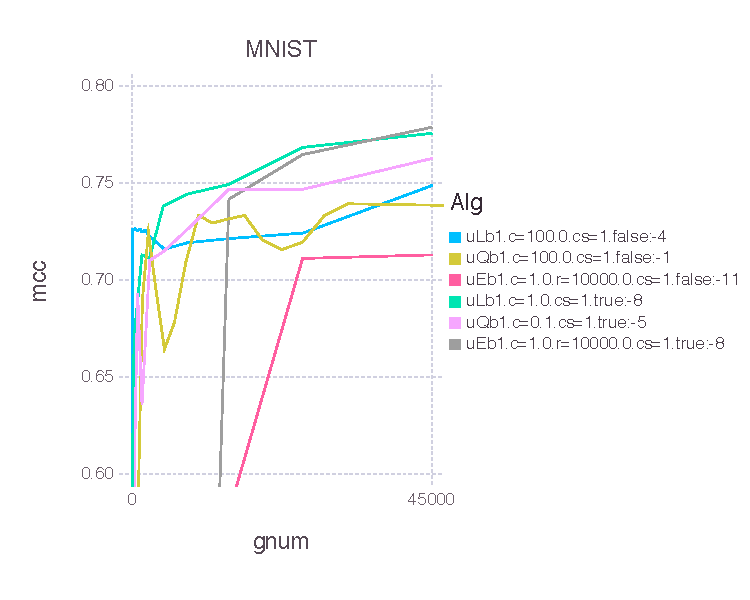
\includegraphics[width= 5in]{Figures/MNISTBLtruemccInitialHeuristics.pdf}
	
	\includegraphics[width= 5in]{Figures/myrandBLtruefInitialHeuristics.pdf}

	\includegraphics[width= 5in]{Figures/myrandBLtruemccInitialHeuristics.pdf}

	\includegraphics[width= 5in]{Figures/alphaGoodBLtruefInitialHeuristics.pdf}

	\includegraphics[width= 5in]{Figures/alphaGoodBLtruemccInitialHeuristics.pdf}

	\includegraphics[width= 5in]{Figures/SUSYBLtruefInitialHeuristics.pdf}

	\includegraphics[width= 5in]{Figures/SUSYBLtruemccInitialHeuristics.pdf}
	
	
	
\end{document} 

